%!TEX root = ../main.tex

\subsection{Local Storage}
Somewhere this should be answered!

How should local data storage be realised?

\subsection{Software on Stationary Computer}
The stationary computer needs to receive data through wifi and decode the received messages using protocol that are to be developed. 
It also has the responsibility of processing data and presenting it to the user in a UI.
The software also needs to have the ability to let the user start and stop specific sensor nodes and send this command to the on-vehicle network. 
The software should run on a Linux OS as an OS eases the task of configuring a wifi network and linux is open-source and is generally used by engineering students.
The described software is outlined in figure \ref{fig:setup_ui}.


\begin{figure}[h]
	\centering
	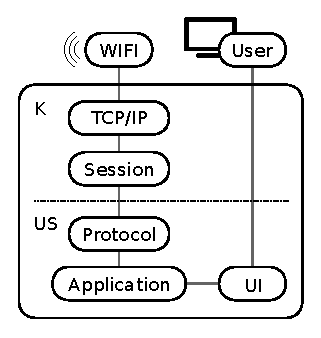
\includegraphics{graphics/stationary_software.eps}
	\caption{Structure of software on stationary computer.}
	\label{fig:setup_ui}
\end{figure}

\subsubsection*{Session}
The software needs to set up a session between the stationary computer and the on-vehicle computer.
\mikkel{Maybe you could add a bit Thomas?}

\subsubsection*{Protocol}
When data is received it needs to be decoded using the developed protocol to recognized what sensor data have been transmitted.


\subsubsection*{Application}
The application could be used to process data in various ways, but it is not the focus of this project.
The application needs to make data available for the UI.
The interface between the application and the UI should be a generic API to ease the development of different UIs. 

\subsubsection*{UI}
As previously stated there needs to be a UI on the stationary computer to let the user monitor the go-kart parameters and start/stop sensors. 
This UI needs to present data in a graphical interface to let the user easily understand the data. 
To develop a sophisticated graphical user interface is not the focus of this project and will therefore be omitted, but a simple UI should be implemented to give the system the wanted functionality shown in the use cases.
